
\documentclass[twocolumn, amsmath]{revtex4}

\usepackage{graphicx}



\begin{document}


\title{PHYS 605 Lab \#9} 

\author{Morgan Daly}
\author{Evin O'Shea}
\date{\today} 


\maketitle


\section{Introduction and Theory}
\subsection{Purpose}

The goal was to build a 4-bit shift register using D flip-flops. This required application of logic concepts to understand the behavior of the D flip-flop.


\subsection{Background / Theory}

A set-reset flip-flop is made up of two NOR (``not or") gates whose output and inputs are connected as shown in figure (1).

\begin{figure}[h]
    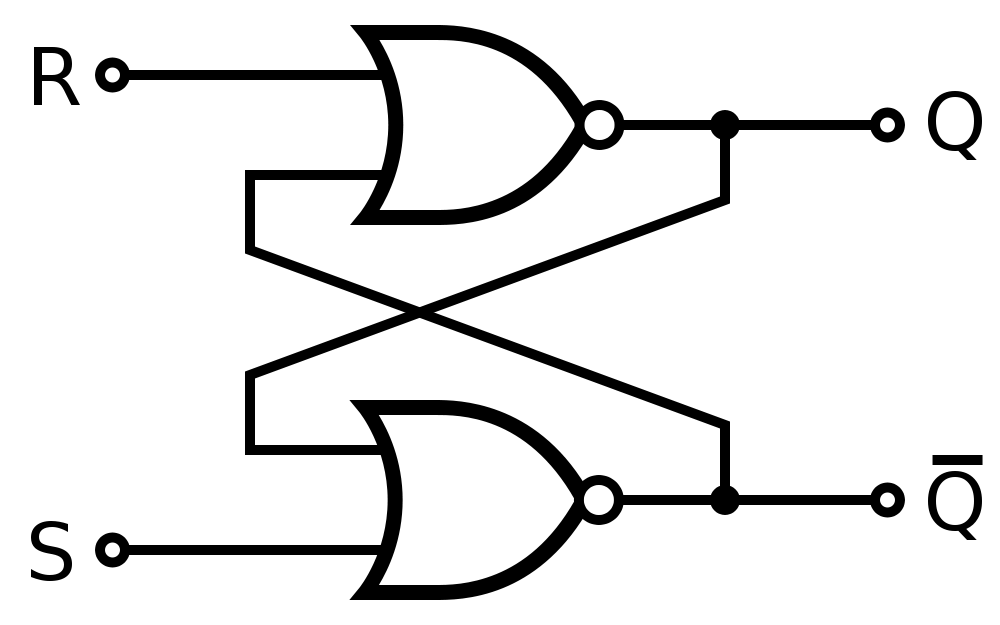
\includegraphics[scale=0.18]{setreset}  
    \caption{A set-reset flip-flop.}
\end{figure}

% could describe the logic here in depth
The output of the set-reset flip-flop is low when S=0 and R=1, and high when S=1 and R=0. The SR flip-flop's truth table is shown below.

\begin{center}
	\begin{ruledtabular}
    \begin{tabular}{ l l l}
	S & R & Q\\ \colrule
	0 & 0 & X \\
	0 & 1 & 0 \\
	1 & 0 & 1
\end{tabular}
    \end{ruledtabular}
\end{center}

A 555 timer is a device which produces timing pulses. The frequency of these pulses depend on the resistor values, $R_a$ and $R_b$, and capacitor value, $C$.

\begin{equation}
f = \frac{1.4}{C(R_a + 2R_b)}
\end{equation}

A D flip flop

\begin{figure}[h]
    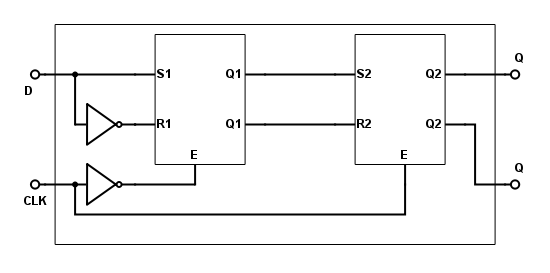
\includegraphics[scale=0.45]{dflipflop}  
    \caption{Detailed view of a D flip-flop.}
\end{figure}

\begin{center}
	\begin{ruledtabular}
    \begin{tabular}{ l l l}
	D & CLK & Q\\ \colrule
	0 & rising edge & 0 \\
	1 & rising edge & 1 \\
\end{tabular}
    \end{ruledtabular}
\end{center}

A shift resistor is a circuit that propagates bits in support of memory management. It takes data in at one terminal, and shifts one bit on each clock pulse that is input to the other terminal.

\begin{figure}[h]
    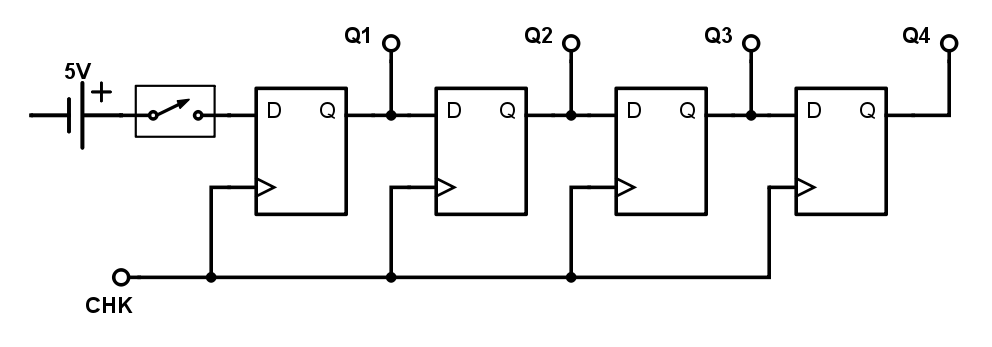
\includegraphics[scale=0.26]{bitshifter.png}  
    \caption{The shift register schematic.}
\end{figure}

Digital circuits consist of different height square pulses that can be categorized as one of two states: high or low, 1 or 0. This type of circuitry is often used in technology because it can send encoded data without error. The error is reduced because a low and high pulse can be easily distinguished even with noise in the signal. This means that the data is only limited by the number of pulses sent.

In the lab, the group used LED's to get a visual feedback on the output of the circuits. 
LED's require a minimum voltage across them to light up. This works well in digital circuits, as the high voltage is over the diode voltage and the low is below it. This means that the LED on is a high coming through and the LED off is as low coming through.

The NAND gate performs the logical operator of ``not and". The truth table for this gate is shown below:


However, when the inputs are connected and therefore the same value, there are only two cases. This truth table is shown below:



When the inputs are tied together, the NAND gate inverts the signal. 

The circuit used in the lab is shown in figure (1). Three NAND gates configured in this way have their own truth table. The inputs to the first two NAND gates will be inverted, due to each terminal receiving the same input. The final NAND gate will have the standard ``not and" behavior shown in the first truth table. The truth table shown below is the equivalent truth table for the three gates:

\begin{center}
	\begin{ruledtabular}
    \begin{tabular}{ l l l}
	IN$_1$ & IN$_2$ & OUT\\ \colrule
	1 & 1 & 1 \\
	1 & 0 & 1 \\
	0 & 1 & 1 \\
	0 & 0 & 0  \\
\end{tabular}
    \end{ruledtabular}
\end{center}

This truth table is equivalent to the truth table of an OR gate. This means the equivalent logical operation for these three gates is ``OR".


Resistors can be used to restrict the current supplied to the NAND gates. The supply voltage in the circuit shown in figure (1) was 5V, so 10k$\Omega$ resistors would result in a 0.5mA current.

A 555 timer is a device which produces timing pulses. A 555 timer can be used to light LEDs alternately; the schematic for this is shown in figure (2). The frequency of these pulses depend on the resistor values, $R_a$ and $R_b$, and capacitor value, $C$.

\begin{equation}
f = \frac{1.4}{C(R_a + 2R_b)}
\end{equation}



This circuit results in alternating lights because of the 555 timer's input to the NAND gate. The other input in is always high, because it is connected directly to the source. The input from the 555 timer alternates between high and low. When the 555 timer is high, both inputs to the NAND gate are high, and the output is low. As a result, the voltage across the first diode is 5V, and the voltage across the second diode is 0V. When the 555 timer is low, the output of the NAND gate will be high, so the voltage across the first diode will be 0V and the voltage across the second diode will be 5 V.

\section{Methodology}

\begin{enumerate}
	\item Using equation (1), select resistor and capacitor values that will create a frequency that makes the circuit behavior easy to observe.
	\item Set up 555 timer.
    \item Construct the shift registor circuit as shown in figure (2). 
    \item Connect an LED to each output Q.
    \item Using the switch to change the input to the circuit, observ
\end{enumerate}


\section{Results and Analysis}

\subsection{Analysis}

The NAND gates operated as expected in the first circuit built. The behavior of the circuit was explained in the background. Since the circuit was digital, the output does not have error, only correct or incorrect output.

The frequency of the flashing lights in the second part of lab was within an expected range. The output frequency only varied from the expected frequency by 0.704\%. Because the percent error was very low, it means the measurements were done accurately and the circuit was built correctly.


\section{Conclusion}

The goal of the first part of the lab was completed successfully. The desired output was obtained and checked during the lab.

For the second part of the lab, the only goal was to obtain a frequency of about 2 Hz. This was achieved with low percent error. This part of the lab was also successfully completed.

\end{document}

